\documentclass[aspectratio=169, table, 12pt]{beamer}

\usepackage{colortbl}
\usepackage{xcolor}
\usepackage{listings}
\usepackage{tabularx}
\usepackage{tikz}
\usetikzlibrary{arrows.meta, positioning, calc, fit, shapes.geometric}

\makeatletter
\def\input@path{{../theme/}}
\makeatother
\graphicspath{{../theme/}{../../figures/}}
\usetheme{Pradita}

\definecolor{praditagreen}{RGB}{37, 113, 71}

% Tema membuat garis tabel berwarna putih. Dikembalikan agar tabel terbaca.
\arrayrulecolor{black}
\setlength{\arrayrulewidth}{0.5pt}

\lstdefinestyle{PythonStyle}{
  language=Python,
  basicstyle=\ttfamily\scriptsize,
  keywordstyle=\color{blue}\bfseries,
  commentstyle=\color{gray}\itshape,
  stringstyle=\color{red},
  breaklines=true,
  frame=lines,
  backgroundcolor=\color{lightgray!10},
  tabsize=2,
  showstringspaces=false
}

\lstdefinelanguage{bash}{
  keywords={},
  basicstyle=\ttfamily\scriptsize,
  ndkeywords={cd, python},
  ndkeywordstyle=\color{purple}\bfseries,
  sensitive=true,
  commentstyle=\color{gray},
  breaklines=true,
  frame=lines,
  backgroundcolor=\color{lightgray!10},
  tabsize=2,
  comment=[l]{\#},
  showstringspaces=false
}

\title{\LARGE{Pertemuan 02:}\\ \Huge{Layered Architecture}}
\subtitle{IF231303 Arsitektur Perangkat Lunak}
\author{Alfa Yohannis}

\begin{document}

\frame{\titlepage}

\begin{frame}{{\Large Tujuan Pembelajaran}}
  \vspace{10pt}
  \begin{enumerate}
    \item Menjelaskan pembagian tanggung jawab keempat lapisan beserta arah
          ketergantungannya.
    \item Membedakan lapisan tertutup dari lapisan terbuka, lalu menentukan
          kapan masing-masing layak dipilih.
    \item Mengukur fungsi penerus, pelanggaran arah, dan selisih waktu antara
          kedua bentuk.
  \end{enumerate}
\end{frame}

\begin{frame}{{\Large Pendahuluan}}
  \vspace{8pt}
  \begin{itemize}
    \item \textit{Layered architecture} menata aplikasi menjadi beberapa
          lapisan yang bertumpuk.
    \item Setiap lapisan mengerjakan satu jenis urusan teknis, lalu memanggil
          lapisan di bawahnya.
    \item Bentuk ini menjadi pilihan pertama bagi sebagian besar sistem, dan
          sering dipakai tanpa pertimbangan panjang.
  \end{itemize}

  \vspace{8pt}
  {\small Alasan pemakaiannya sering bersifat organisasi, bukan teknis.
  Pembagian lapisan mengikuti pembagian kerja yang sudah ada di banyak tim,
  yaitu ada yang mengerjakan antarmuka, ada yang mengerjakan aturan bisnis, dan
  ada yang mengerjakan basis data.}

  \vspace{6pt}
  {\small Kemudahan itu ada harganya. Ketika aplikasi membesar, satu fitur baru
  sering menyentuh keempat lapisan sekaligus.}
\end{frame}

\begin{frame}{{\Large Contoh Isi Setiap Lapisan}}
  \vspace{6pt}
  \centering
  \small
  \begin{tabularx}{0.97\textwidth}{|l|X|X|}
    \hline
    \textbf{Lapisan} & \textbf{Contoh isinya} & \textbf{Kalimat kebutuhan} \\
    \hline
    Presentasi & Menyusun teks \texttt{100 USD = 1.625.000 IDR} & Hasil ditampilkan dengan pemisah ribuan \\
    \hline
    Bisnis & Menolak nominal nol, memeriksa token dan peran & Hanya staf boleh melihat kurs jual \\
    \hline
    Persistensi & Mengubah baris tabel menjadi tupel & Kurs disimpan per pasangan mata uang \\
    \hline
    Basis Data & Tabel \texttt{kurs} beserta kolom \texttt{margin} & Margin disimpan terpisah dari nilai referensi \\
    \hline
  \end{tabularx}

  \vspace{10pt}
  {\small Uji cepat: bila sebuah kebutuhan tetap berlaku walaupun layar diganti
  menjadi API, kebutuhan itu milik lapisan bisnis.}
\end{frame}

\begin{frame}{{\Large Empat Lapisan Baku}}
  \vspace{5pt}
  \centering
  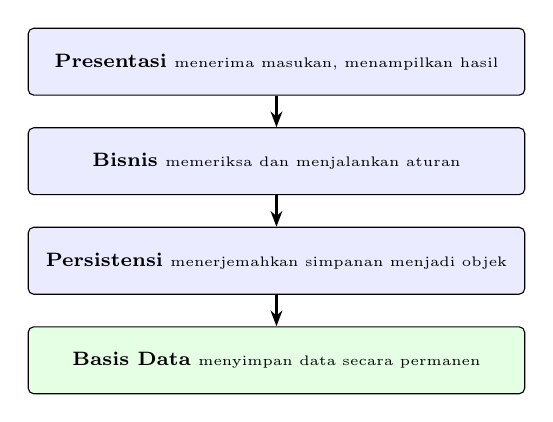
\begin{tikzpicture}[
    lapis/.style={draw, rounded corners=2pt, minimum width=0.52\textwidth,
      minimum height=0.85cm, align=center, font=\scriptsize},
    panah/.style={-{Stealth[length=2mm]}, thick}
  ]
    \node[lapis, fill=blue!8] (pres) {\textbf{Presentasi}
      {\tiny\mdseries menerima masukan, menampilkan hasil}};
    \node[lapis, fill=blue!8, below=0.4cm of pres] (bis) {\textbf{Bisnis}
      {\tiny\mdseries memeriksa dan menjalankan aturan}};
    \node[lapis, fill=blue!8, below=0.4cm of bis] (per) {\textbf{Persistensi}
      {\tiny\mdseries menerjemahkan simpanan menjadi objek}};
    \node[lapis, fill=green!10, below=0.4cm of per] (bas) {\textbf{Basis Data}
      {\tiny\mdseries menyimpan data secara permanen}};
    \draw[panah] (pres) -- (bis);
    \draw[panah] (bis) -- (per);
    \draw[panah] (per) -- (bas);
  \end{tikzpicture}

  \vspace{8pt}
  {\small Panggilan hanya boleh mengarah ke bawah, dan tidak boleh melompat.}
\end{frame}

\begin{frame}{{\Large Dua Konsekuensi Aturan Tersebut}}
  \vspace{10pt}
  \begin{itemize}
    \item Satu lapisan dapat diganti tanpa menyentuh lapisan lain, selama
          bentuk panggilannya tetap. Jadi, tidak perlu mengubah lapisan lain.
    \item Permintaan sederhana tetap harus melewati seluruh lapisan, walaupun
          sebagian lapisan tidak mengerjakan apa pun.
  \end{itemize}

  \vspace{10pt}
  {\small Konsekuensi kedua menimbulkan pertanyaan berikutnya, yaitu apakah
  setiap permintaan benar-benar wajib melewati semua lapisan.}
\end{frame}

\begin{frame}{{\Large Lapisan Tertutup dan Lapisan Terbuka}}
  \vspace{5pt}
  \centering
  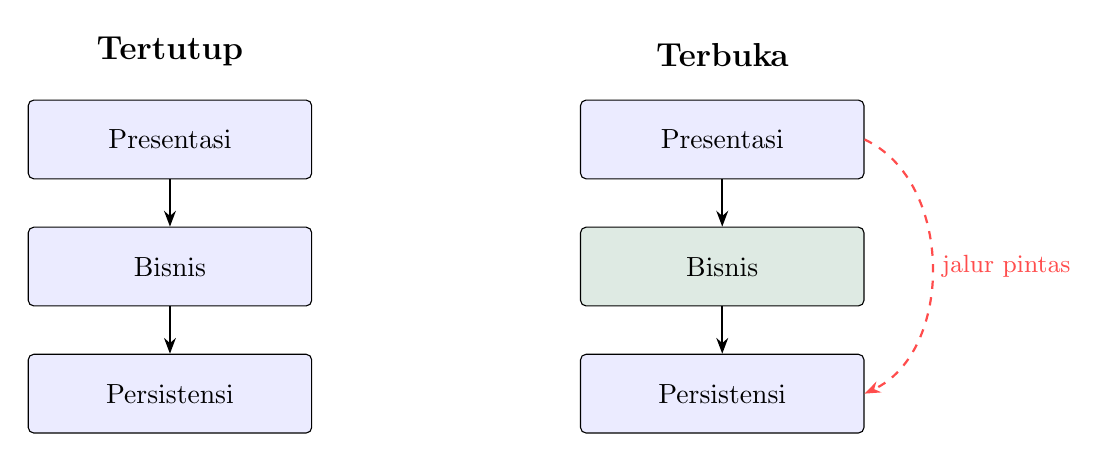
\begin{tikzpicture}[
    lapis/.style={draw, rounded corners=2pt, minimum width=3.6cm,
      minimum height=1.0cm, align=center, font=\normalsize},
    panah/.style={-{Stealth[length=2mm]}, thick},
    lompat/.style={-{Stealth[length=2mm]}, thick, red!70, dashed}
  ]
    \node[lapis, fill=blue!8] (p1) {Presentasi};
    \node[lapis, fill=blue!8, below=0.6cm of p1] (b1) {Bisnis};
    \node[lapis, fill=blue!8, below=0.6cm of b1] (s1) {Persistensi};
    \node[font=\large\bfseries, above=0.3cm of p1] {Tertutup};
    \draw[panah] (p1) -- (b1);
    \draw[panah] (b1) -- (s1);

    \node[lapis, fill=blue!8, right=3.4cm of p1] (p2) {Presentasi};
    \node[lapis, fill=praditagreen!15, below=0.6cm of p2] (b2) {Bisnis};
    \node[lapis, fill=blue!8, below=0.6cm of b2] (s2) {Persistensi};
    \node[font=\large\bfseries, above=0.3cm of p2] {Terbuka};
    \draw[panah] (p2) -- (b2);
    \draw[panah] (b2) -- (s2);
    \draw[lompat] (p2.east) to[out=-25, in=25]
      node[right, font=\small] {jalur pintas} (s2.east);
  \end{tikzpicture}
\end{frame}

\begin{frame}{{\Large Architecture Sinkhole}}
  \vspace{10pt}
  \begin{itemize}
    \item Permintaan mengalir melewati beberapa lapisan tanpa satu pun lapisan
          mengerjakan sesuatu.
    \item Keadaan ini hampir tidak mungkin dihapus, sehingga yang diusahakan
          adalah menekan jumlahnya.
    \item Yang diperiksa adalah apakah lapisan bisnis lebih sering meneruskan
          panggilan daripada mengerjakan sesuatu.
    \item Lapisan mana yang tertutup dan mana yang terbuka wajib dicatat dan
          disepakati satu tim.
  \end{itemize}
\end{frame}

\begin{frame}[fragile]{{\Large Penerus yang Wajar dan yang Tidak}}
  \vspace{5pt}
\begin{lstlisting}[style=PythonStyle]
def susun_kurs_referensi():
  # Kurs referensi memang diterbitkan untuk umum, meniru JISDOR.
  # Tidak ada tuntutan bisnis, sehingga fungsi ini murni penerus.
  return daftar_kurs_referensi()

def susun_kurs_jual(token):
  # Kurs jual memuat margin, dan margin bersifat komersial.
  # Lapisan bisnis menuntut dua pemeriksaan sebelum data diberikan.
  pengguna = autentikasi.periksa_token(token)
  if pengguna is None:
    raise PermissionError("Token tidak dikenali")
  if not autentikasi.boleh_membaca(pengguna):
    raise PermissionError("Peran tidak berhak membaca kurs jual")
  return daftar_kurs_jual()
\end{lstlisting}

  \vspace{3pt}
  {\small Jalan pintas pada yang pertama wajar. Pada yang kedua, dua
  pemeriksaan ikut hilang.}
\end{frame}

\begin{frame}{{\Large Analogi: Tiga Meja dan Satu Cap}}
  \vspace{10pt}
  \begin{itemize}
    \item Surat pengantar harus melewati tiga meja sebelum disetujui.
    \item Meja pertama membaca isinya lalu memutuskan.
    \item Meja kedua dan ketiga hanya membubuhkan cap, lalu meneruskan.
    \item Ketiganya menambah waktu, tetapi hanya satu menambah nilai.
  \end{itemize}

  \vspace{10pt}
  {\small Prosedurnya terlihat rapi di atas kertas, tetapi dua meja terakhir
  adalah \textit{sinkhole}. Itulah yang terjadi pada lapisan yang hanya
  meneruskan panggilan.}
\end{frame}

\begin{frame}{{\Large Kasus: Jalan Pintas yang Dipakai Ulang}}
  \vspace{8pt}
  \begin{enumerate}
    \item Tim menambah halaman perbandingan kurs untuk pengunjung umum.
    \item Halaman dibangun cepat dengan memanggil lapisan persistensi langsung.
    \item Keputusan itu benar, sebab yang ditampilkan hanya kurs referensi.
    \item Beberapa bulan kemudian kurs jual diminta muncul di halaman yang sama.
    \item Fungsinya tinggal diganti, sebab jalurnya sudah terbuka.
  \end{enumerate}

  \vspace{8pt}
  {\small Sejak saat itu margin terbaca siapa pun. Tidak ada galat yang muncul,
  sehingga tidak ada yang menyadarinya.}
\end{frame}

\begin{frame}{{\Large Hasil Pengukuran}}
  \vspace{8pt}
  \centering
  \small
  \begin{tabularx}{0.92\textwidth}{|X|l|l|}
    \hline
    \textbf{Berkas} & \textbf{Fungsi penerus} & \textbf{Pelanggaran arah} \\
    \hline
    \texttt{aplikasi\_tertutup} & 1 dari 12, yaitu 8,3 persen & 0 \\
    \hline
    \texttt{aplikasi\_terbuka} & 0 dari 6 & 2 \\
    \hline
  \end{tabularx}

  \vspace{12pt}
  \begin{tabularx}{0.92\textwidth}{|X|l|}
    \hline
    \textbf{Kurs jual, seratus putaran} & \textbf{Nilai} \\
    \hline
    Median jalur tertutup, dengan pemeriksaan & 0,0810 ms \\
    \hline
    Median jalur terbuka, tanpa pemeriksaan & 0,0776 ms \\
    \hline
    Selisih median & $-0,0035$ ms \\
    \hline
    Putaran dimenangkan jalur terbuka & 91 dari 100 \\
    \hline
  \end{tabularx}

  \vspace{8pt}
  {\small Jalan pintas memang lebih cepat, sekitar empat persen. Kecepatan itu
  dibeli dengan melewati autentikasi dan otorisasi.}
\end{frame}

\begin{frame}{{\Large Ringkasan}}
  \vspace{10pt}
  \begin{itemize}
    \item Empat lapisan, satu aturan, yaitu panggilan hanya mengarah ke bawah.
    \item Aturan itu menahan perubahan di satu lapisan, tetapi memaksa
          permintaan sederhana melewati lapisan yang tidak bekerja.
    \item Fungsi penerus ditekan jumlahnya, bukan dihapus sepenuhnya.
    \item Lapisan terbuka memangkas kode penerus, tetapi menambah dua
          pelanggaran arah ketergantungan.
    \item Jalan pintas terbukti lebih cepat, yaitu menang 91 dari 100 putaran,
          sebab dua pemeriksaan tidak dijalankan.
    \item Yang menentukan bukan kecepatan, melainkan ada tidaknya tuntutan
          bisnis yang ikut dilewati.
  \end{itemize}
\end{frame}

\begin{frame}[fragile]{{\Large Persiapan Latihan}}
  \vspace{5pt}
\begin{lstlisting}[language=bash]
cd sources/chapter02
python basis_data.py
\end{lstlisting}

  \vspace{8pt}
  {\small Satu basis kode, tiga masalah berbeda. Aplikasi melayani dua
  permintaan pada tabel yang sama, yaitu kurs referensi yang publik dan kurs
  jual yang memuat margin.}
\end{frame}

\begin{frame}[fragile]{{\Large Latihan 1: Menghitung Fungsi Penerus}}
  \vspace{3pt}
\begin{lstlisting}[language=bash]
python periksa_lapisan.py aplikasi_tertutup.py
python periksa_lapisan.py aplikasi_terbuka.py
\end{lstlisting}

  \vspace{3pt}
  \begin{enumerate}
    \item Catat baris \texttt{Fungsi penerus} dan \texttt{Bagian penerus}.
    \item Buka kedua berkas, lalu periksa tubuh fungsi yang dilaporkan
          sebagai penerus.
    \item Nilai apakah lapisan bisnis lebih banyak bekerja daripada
          meneruskan.
  \end{enumerate}

  \vspace{3pt}
  {\small Pertanyaan: satu-satunya penerus yang tersisa melayani kurs
  referensi. Mengapa keberadaannya tetap dapat dibenarkan?}
\end{frame}

\begin{frame}[fragile]{{\Large Latihan 2: Menemukan Pelanggaran Arah}}
  \vspace{3pt}
\begin{lstlisting}[language=bash]
python periksa_lapisan.py aplikasi_terbuka.py
python aplikasi_terbuka.py
python aplikasi_tertutup.py USD IDR 100
\end{lstlisting}

  \vspace{3pt}
  \begin{enumerate}
    \item Catat baris \texttt{Pelanggaran arah} pada kedua berkas.
    \item Perhatikan bahwa kurs jual terbaca tanpa token apa pun pada versi
          terbuka.
    \item Bandingkan perlakuannya terhadap token yang tidak dikenali pada
          versi tertutup.
  \end{enumerate}

  \vspace{3pt}
  {\small Pertanyaan: kedua pelanggaran tidak sama beratnya. Mana yang dapat
  dibenarkan, dan mengapa?}
\end{frame}

\begin{frame}[fragile]{{\Large Latihan 3: Mengukur Biaya Pemeriksaan}}
  \vspace{3pt}
\begin{lstlisting}[language=bash]
python ukur_lapisan.py
\end{lstlisting}

  \vspace{3pt}
  \begin{enumerate}
    \item Perhatikan bahwa skrip menjalankan seratus putaran, bukan satu.
    \item Catat keenam angka yang dilaporkan.
    \item Bandingkan selisih median antar jalur dengan ragam di dalam satu
          jalur.
    \item Bandingkan jumlah kemenangan jalur terbuka dengan lima puluh.
  \end{enumerate}

  \vspace{3pt}
  {\small Pertanyaan: hitung penghematannya dalam persen, lalu bandingkan
  dengan tuntutan bisnis yang dilepas.}
\end{frame}

\end{document}
